\documentclass[twocolumn]{article}
\usepackage[utf8]{inputenc}
\usepackage[T1]{fontenc}
\usepackage[english]{babel}
\usepackage{diagbox}
\usepackage{ifpdf,amsmath,amsthm,amssymb,amsfonts,newtxtext,newtxmath} 
\usepackage{array,graphicx,dcolumn,multirow,hevea,abstract,hanging}
\usepackage[labelfont=sc,textfont=sf]{caption}
\usepackage[hyperfootnotes=false,breaklinks=true]{hyperref} % was dvipdfmx
\urlstyle{rm}
%\usepackage[hyphenbreaks]{breakurl}
\usepackage{apacite} % must come afer hyperfootnotes
\setlength{\bibleftmargin}{1em}
\setlength{\bibindent}{-1em}
\usepackage{booktabs} % \toprule \midrule \bottomrule \cmidrule(lr){a-b}

%%%% Added by Zhenbo Cheng
\usepackage{subcaption}
%%%%%%%%%%%%%%%%%%%%%%%%

% define centered and ragged columns:
\newcolumntype{L}[1]{>{\raggedright\arraybackslash }p{#1}} % can use m{}
\newcolumntype{C}[1]{>{\centering\arraybackslash }p{#1}}
\newcolumntype{R}[1]{>{\raggedleft\arraybackslash }p{#1}}
\newcolumntype{d}[1]{D{.}{.}{#1}} % d{3.2} for 3 places on l, 2 on r
\newcommand{\mc}{\multicolumn}
\topmargin=-.3in \oddsidemargin=-.1in \evensidemargin=-.1in \textheight=9in \textwidth=6.8in
\setlength\tabcolsep{1mm}
\setlength\columnsep{5mm}
\setlength\abovecaptionskip{.5ex}
\setlength\belowcaptionskip{.5ex}
\setlength\belowbottomsep{.3ex}
\setlength\lightrulewidth{.04em}
\renewcommand\arraystretch{1.2}
\renewcommand{\topfraction}{1}
\renewcommand{\textfraction}{0}
\renewcommand{\floatpagefraction}{.9}
% \renewcommand{\baselinestretch}{1.00} \large\normalsize % for fixing spaces
\widowpenalty=1000
\clubpenalty=1000
\setlength{\parskip}{0ex}
\let\tempone\itemize
\let\temptwo\enditemize
\let\tempthree\enumerate
\let\tempfour\endenumerate
\renewenvironment{itemize}{\tempone\setlength{\itemsep}{0pt}}{\temptwo}
\renewenvironment{enumerate}{\tempthree\setlength{\itemsep}{0pt}}{\tempfour}

%%%%%%%%%%%%%%%%%%%%%%%%%%%%%%%%%%%%%%%%%%%%%%%%%%%%%%%%%%%%%%%%%%%%%
\setcounter{page}{1} % start with first page

\title{Title}

\author{
Zhenbo Cheng\thanks{Department of Computer Science and Technology, Zhejiang University of Technology, Hangzhou, China}\;\,
\and
    Gang Xiao\footnotemark[1]\thanks{Email: xg@zjut.edu.cn}\;\,
}

% who is corresponding author?

\date{} % leave empty
\begin{document} % goes here

% fill in short title
\newcommand{\jref}{http://journal.sjdm.org/vol13.2.html}
\newcommand{\jhead}{Judgment and Decision Making, Vol.~13, No.~2}
\newcommand{\jdate}{March 2018}
\pagestyle{myheadings} \markright{\protect\small \href{\jref}{\jhead}, \jdate \hfill Strategies of matcching and maxmizing \qquad}
\begin{htmlonly}
\href{\jref}{\jhead}, \jdate, pp.\
\end{htmlonly}
%\begin{latexonly}
\twocolumn[
\vspace{-.3in}
{\small \href{\jref}{\jhead}, \jdate, pp.\ XX--XX}
%\end{latexonly}

\maketitle

%\begin{latexonly}
\vspace{-3mm}
\begin{onecolabstract}
%\end{latexonly}
In recent years, the increasing demand for seamless switching of HD streams and the
 widespread adoption of adaptive streams based on the DASH standard have become the 
main driving force for the research of rate adaptive algorithms.
Most of the existing bit rate adaptive algorithms are hard-coded and 
cannot effectively cope with changes in the network environment.
In addition, some scholars have proposed to use the Q learning method that 
can obtain higher QoE to learn the optimized code rate adaptive algorithm.
However, Q learning has the problem that it is difficult to encode continuous 
state values and the algorithm converges slowly in large state spaces.
To this end, this paper combines the nearest neighbor algorithm and proposes a 
KNN-Q learning algorithm that can handle continuous state.
The experimental results show that in the rate adaptive scenario, 
KNN-Q learning can achieve higher QoE and faster convergence speed than 
ordinary Q learning.

\smallskip
\noindent
Keywords: DASH, HTTP adaptive streaming, reinforcement learning,Q learning,KNN
%\begin{latexonly}
\end{onecolabstract}\bigskip
]
%\end{latexonly}

{\renewcommand{\thefootnote}{}
\footnotetext{ % note blank lines above and below acknowledgment

    This work is supported by Public Projects of Zhejiang Province
    (2016C31G2020069) and the 3rd Level in Zhejiang Province “151
    talents project” to Zhenbo Cheng. We thank Liwen Bianji, Edanz Group
    China (www.liwenbianji.cn/ac), for editing the English text of a
    draft of this manuscript. The authors declare no competing financial
    or nonfinancial interests.

Copyright: \copyright\ 2018.
The authors license this article under the terms of the
\href{http://creativecommons.org/licenses/by/3.0/}{Creative Commons
    Attribution 3.0 License.}
}}

\saythanks

\setlength{\baselineskip}{12pt plus.2pt}

\section{Introduction}
At present, video data is becoming the mainstream data of the traditional Internet, 
especially the mobile Internet.Video data requires a higher bit rate than other 
data transmissions, and the resulting increase in mobile traffic is more pronounced.
According to the Cisco Global Mobile Data Traffic Forecast Update white paper(2016- 2021)\cite{RN1}, 
mobile video flow will grow 8.7 times by 2021, accounting for 78\% of total mobile traffic.
Users have more requirements for video quality and interactive features.

Thousands of videos are transmitted over HTTP every day.
Video data can be easily transmitted through HTTP and NAT devices.
Based on HAS (HTTP Adaptive Streaming) technology, major vendors have developed adaptive 
streaming media technologies for their respective devices or clients, such as 
Apple's HLS (HTTP Live Streaming) , Microsoft's MSS (Microsoft Silverlight Smooth Streaming) 
and Adobe's HDS (HTTP Dynamic Streaming).
The MPEG organization developed the DASH (Dynamic Adaptive Streaming over HTTP) standard 
in 2011 to unify the video technology standards for transmitting dynamic bitrates between 
different device and server manufacturers\cite{RN2}.Compared with HLS and MSS, 
the DASH standard not only supports multiple encoding methods, 
but also supports CDN docking from multiple manufacturers.

The design of the DASH standard is that the server divides the original video 
into video clips with the same content and 
different bit rates, and then generates an index file MPD (Media Presentation Description) 
containing all the video clip information and their download addresses.
After the client downloads and parses the MDP file, it switches the 
video clip of the appropriate bit rate according to the current video 
quality and network conditions during playback\cite{RN3}.
The DASH standard opens up the design of the bit rate adaptive algorithm, 
enabling developers to implement their own rate adaptive algorithms to 
provide higher QoE (Quality of Experience).

The existing bit rate adaptive algorithms are mostly based on heuristic algorithms. 
The algorithm usually uses hard coding to select the appropriate bit rate according 
to the network conditions, which may result in the inability to effectively
 cope with the frequent fluctuations of the network environment\cite{RN4}.
 Dana et al. proposed a Q-Learning algorithm in reinforcement 
 learning to obtain an optimized bit rate adaptive strategy\cite{RN5}.
 Compared with the heuristic algorithm, this method can obtain higher QoE, 
 but when the state is divided too much, the method has the difficulty
  of learning continuous state values and slow learning convergence.
Aiming at this problem, this paper proposes a KNN-Q learning algorithm 
as a strategy for obtaining video clips in combination with the 
nearest neighbor algorithm.The experimental results 
show that the KNN-Q learning algorithm can achieve higher QoE.

\section{Related work}
The client downloads streaming media and must be able to adaptively select 
the bit rate according to the network situation, client state and user experience, 
in order to play video reliably and efficiently in different environments.

Studies\cite{RN7} have shown that users are not sensitive 
to the improvement of image quality, but often can detect the decline in image quality.
The algorithm should try to avoid changing the image quality frequently. 
Even if the image quality change cannot be avoided, 
algorithm need to control changes within a small range.
QoE-related adaptive strategies often need to consider multiple aspects 
such as available bandwidth, buffer, quality, etc. to accurately reflect the QoE perceived by the user.
Mok et al\cite{RN6}. proposed a heuristic-based bit rate adaptive algorithm combined with QoE.
 The QDASH-abw module is located in the proxy of the server to measure the highest video quality 
 that can be supported under the current bandwidth. 
 The client selects the most suitable video quality rate based on the QDASH-qoe algorithm.
 Their experimental results indicate that users prefer a smooth 
 transition between the best and worst video quality, rather than a sudden switch.
 Zink et al\cite{RN7}.'s NOVA adaptive strategy proposes that "cross-layer" is designed to 
 weigh resource allocation and rate adaptation, using the variance of the quality 
 and time of the previous S video segments as a measure of QoE.
 The heuristic-based rate adaptive algorithm cannot easily establish a predictable mathematical model. 
 And,the flexibility of the bit rate selection strategy is low. 
 In the complex network environment, the stability of the this algorithm is poor.

 Using machine learning methods, the client can learn how to adjust the bit 
 rate of the requested video block based on changes in the context before and after intervention.
 Using machine learning methods can enhance the adaptability and flexibility of the client's rate adaptive strategy.
 Based on the random forest decision tree model, Chien et al\cite{RN9}. map network state eigenvalues 
 (such as the bandwidth of the latest slice, the average bandwidth of the session, and the fluctuation of the bandwidth) 
 to the bit rate label obtained by the other excellent bit rate adaptive algorithm. 
 Finally, the trained classification model is used to predict the bit rate size of the video segment.
 One disadvantage based on supervised learning is the need to prepare training data. 
 Although Chien's algorithm can collect user data through online learning methods, 
 it is difficult to train a robust model for all scenes due to the environment, 
 user requirements and the diversity of terminal devices.

 Introducing reinforcement learning into the DASH bit rate adaptive algorithm, 
 the HAS client can continuously interact with the environment, 
 train its own strategy according to the feedback of the current network 
 environment, and dynamically learn to select the best action.
 Compared to supervised learning, reinforcement learning does not require a 
 large amount of training data to be prepared, and only a reasonable 
 action reward function needs to be defined during learning.
 Marinca et al\cite{RN10}. implemented a HAS self-learning system on the MAC layer. 
 The system uses a partially visible Markov model to model a bit rate adaptive algorithm based on Q learning.
 Zhu et al\cite{RN11}. proposed an infinite time Markov model, 
 using the Virutal Experience (VR) strategy to update the Q table during training.
 The experimental results of they proposed method show that the VR strategy accelerates 
 the process of model convergence. Compared with the approximate optimal heuristic algorithm,
  thier overall reward is higher and the delay is significantly reduced in the environment with changing network state.
Zhang et al\cite{RN12}. positioned QoE criteria as total cumulative bit rate, 
packet loss rate and video starvation duration, and constructed a 
deep self-transfer learning network (STL) considering QoE.
The STL algorithm integrates a series of pseudo-rewards to train the virtual decision-making center.
Then the virtual decision-making center continuously passes the learned adaptive 
decision to the original decision-making center. The experimental results show that the STL 
algorithm can improve the training efficiency and generalization performance.
After combining the characteristics of deep learning and reinforcement learning, 
Gadaleta et al\cite{RN14}. used the advantages of feedforward neural network and recurrent neural network to design a D-DASH framework.
The D-Dash framework uses video clip quality and video replay event 
evaluation performance to achieve a fairly high QoE in both simulated and real-world environments.

In the context of using reinforcement learning to solve rate adaptation, 
it is necessary to weigh the algorithm convergence speed and state partition granularity.
Too many states can enhance the robustness of the system, 
but it will cause the convergence speed to be too slow in the iteration; 
If the state division is too discrete, and the problem situation cannot 
be drawn to the ideal state, but the convergence speed is accelerated.
In the adaptive rate scene, the states are continuous values. 
This paper proposes an algorithm combining k-nearest neighbor and Q-learning.
Considering the video quality of streaming media, three aspects related to 
QoE are comprehensively selected: the quality of video clips, 
the quality of video frames before and after, and the risk of buffer 
overflow construction to construct a reward function.
In this paper, an algorithm based on KNN Q-learing for bit rate adaptive action of continuous state is implemented,
 and a simulation experiment is designed to compare the performance of 
 ordinary Q learning and KNN-Q learning.
\section{KNN-Q algorithm}
A normal timing-based DASH client will use the discovery strategy to select 
the appropriate bitrate when requesting the next video segment. 
As used herein, an agent based on reinforcement learning which help DASH client
 to make decisions to complete this process of exploration.

Reinforcement learning is a kind of machine learning. 
Because the environment is partially visible to the agent, the uncertainty of the 
agent's response to the environment is determined. 
But interacting with the environment is the only way for an agent to learn and grow. 
The agent receives rewards from the environment after each step of the action, 
and the agent understands the reward and makes the next decision. 
The goal of the agent is to pick the best action among the given environments to maximize the cumulative rewards\cite{RN13}.

In the bit rate adaptive algorithm, the DASH client is defined as an agent, 
and the environment value observed by the agent is defined as the state s. 
The DASH client requests the download of the video segment of a certain 
bit rate as action a at a certain time.
When agent start exploring, it updates the state of the current environment.
In Q learning, the Q table is equivalent to the brain of the agent to help the agent make decisions. 
The Q function is used to evaluate the quality of each action in the current state.
As shown in equation \ref{q table update rule}, the agent selects action a in state s,
and how to update the Q value after obtaining the reward r given by the environment.
Where $\eta\in\left[0;1\right]$ is the learning rate, representing the extent to which the new value replaces the old value;
 $\lambda\in\left[0;1\right]$as a discount factor, measure the importance of future rewards.
 In the case of the state of the environment division meticulous, 
 using this method to update Q table will bring convergence speed is too slow.
 The environment state in the bit rate adaptive context is a continuous value. 
 Based on the KNN algorithm, this paper updates several consecutive states of 
 the current environmental state according to certain strategies, 
 which can achieve the effect of speeding up the iteration rate and obtaining higher cumulative rewards(see section 3.4).
\begin{equation}
\label{q table update rule}
\begin{aligned}
&\left(1-\eta\right)Q_{old}\left(s_t,a_t\right)+\eta\left[r_{t+1}+\lambda max Q\left(s_{t+1},a\right)\right]\\    
&\Rightarrow Q_{new}\left(s_t,a_t\right)
\end{aligned}
\end{equation}

In each training iteration agent selects the appropriate bit rate video clip to download 
according to the previously learned Q value. For the specific selection strategy(see section 3.3),
the reward given by the current action of the environment is calculated based on the reward function (see section 3.2).
After multiple iterations of training, a convergent Q table is generated. 
When the DASH client selects the appropriate bit rate to download the video according to 
the final generated Q table . 
After downloading the current video clip, the video clip will be added to the buffer queue to deal with 
special cases such as network anomalies, and finally the video queue will be played.
\section{Environment model}
The DASH client needs to collect the currently visible environment state 
to build the corresponding reward function and act according to the 
corresponding policy. The following describes the environment state and defines the action behavior of the DASH client.
\subsubsection{Environment status}
This article uses three state components to define the state of the environment: the available bandwidth,
 the total length of the buffer, and the video quality of the previous video clip. 
 The available bandwidth is measured by the DASH client; 
 the total duration of the buffer represents the padding status of the 
 video clip bufferd by the DASH client.
 The state of the final synthesis of these three state components defines $s_t=(BW_t,B_t,q_t-1)$. 
 The value range and discrete level of the specific state component are shown in Table \ref{environment state}.
\begin{table}[h]
\centering
\renewcommand\arraystretch{0.8}
\caption{Environment state definition}
\label{environment state}
\begin{tabular}{ccc}
\toprule
Status element& Range& Level\\
\midrule
Bandwidth& $\left[0;BW_{max}\right]bps$& $N+1$\\
Buffer filling& $\left[0;B_{max}\right]sec$& $\frac{B_{max}}{T_{seg}}$\\
Quality Level(SSIM)&$\left[-1;1\right]$&$N$\\
\bottomrule
\end{tabular}
\end{table}

As shown in Table \ref{environment state}, $BW_{max}$ represents the highest available bandwidth, 
$B_{max}$ represents the maximum video length that can be stored in the buffer area,
 and $N$ represents the total number of bit rate levels. 
 The calculation method of the quality of the previous video 
 clip is evaluated by SSIM (for the calculation method, see section 3.2.1).
 \subsubsection{Selection action}
 The action of the DASH client is defined to request downloading of a video clip of a certain bit rate.
The download rate of the video clip that can be selected by the DASH client is determined in advance 
by the transcoding module of the DASH client.
\subsection{Reward function}
In reinforcement learning, the reward function is the basic guide to the experience of the agent's learning strategy. 
In the streaming adaptive context, the reward function is generally used to measure QoE, 
but the evaluation of QoE is often subjective. For example, it is impossible to compare a video 
that fluctuates between high and low quality and a video that is stable in medium quality. 
So it is necessary to use mathematical models to accurately measure QoE. 
This paper constructs a reward function from three aspects: current video clip quality, 
video clip quality fluctuation and buffer overflow risk.
\subsubsection{Video quality}
This article uses SSIM, which is widely used to evaluate video quality, 
as an indicator for evaluating video quality\cite{RN15,RN16,RN17}.
SSIM is an indicator that measures the similarity of two images and 
uses structural information to evaluate image quality.
The specific calculation of SSIM is as shown in equation \ref{SSIM calculation function}. 
For a given image $X$ and $Y$, the SSIM value is calculated using the mean, 
variance and covariance of the pixel brightness in the two images.
Where $\mu_{X}$ and $\mu_{Y}$ are the average brightness of the pixels of the 
images $X$ and $Y$, $\sigma_{X}^2$ and $\sigma_{Y}^2 $ is the variance of the pixel brightness 
values of the images $X$ and $Y$, respectively, and $\sigma_{XY}$ is the covariance between 
the pixel brightness values of the images $X$ and $Y$, $c_{1 }$ and $c_{2}$ are constants 
set to avoid the denominator being zero.
SSIM$\in\left[-1,1\right]$, the closer value of SSIM is to 1, the higher the similarity between the two images.
\begin{equation}
\label{SSIM calculation function}
SSIM\left(X,Y\right)=\frac{\left(2\mu_{X}\mu_{Y}+c_{1}\right)\left(2\sigma_{XY}+c_{2}\right)}
{\left(\mu_{X}^2+\mu_{Y}^2+c_{1}\right)\left(\sigma_{X}^2+\sigma_{Y}^2+c_{2}\right)}
\end{equation}

Using equation \ref{SSIM calculation function}, the SSIM mean of each video frame of the video clip to be 
downloaded and the original video clip is calculated to measure the 
quality of the video clip. 
As shown in equation \ref{q_n}, the quality of the video clip is represented by the average SSIM of the video clip, 
where $m$ indicates that the video clip is composed of $m$frame pictures, and $q_{n}$ 
indicates the video quality of the nth clip.
\begin{equation}
\label{q_n}
q_{n}=\frac{\sum_{i=0}^m SSIM(download_{seg(i)},origin_{seg(i)})}{m}
\end{equation}

As shown in equation \ref{R_q}, the video quality of the nth segment is used to represent the reward value 
brought by the DASH client downloading the video segment of the video quality.
\begin{equation}
\label{R_q}
R_{quality}=q_{n}
\end{equation}
\subsubsection{Video quality oscillation}
When the network bandwidth changes, the video quality requested by the DASH client also changes, 
and the video quality oscillation will bring about a drop in QoE. As shown in equation\ref{R_quality_change}, 
the reward loss due to quality switching during video playback is recorded as $R_{quality-change}$, 
which is mapped to a penalty reward based on the oscillating step size $\alpha$.
\begin{equation}
\label{R_quality_change}
R_{quality-change}=-\alpha\left|q_{n}-q_{n-1}\right|
\end{equation}
\subsubsection{Buffer security}
The penalty item is set in this paper to measure the buffer security. 
As shown in equations \ref{R_buffer_filling}, \ref{R_buffer_safe}, and \ref{R_buffer_low}, 
the penalty item consists of a secure buffer level penalty and a low buffer penalty.
 Where $B_{max}$ represents the maximum buffer size of the buffer, and $B_{n}$ represents the 
 length of the video clip owned by the buffer when the nth video clip is downloaded. 
 $\beta$ and $\gamma$ represent the focus on buffer security and low buffer.
\begin{equation}
\label{R_buffer_filling}
R_{buffer-filling}=R_{buffer-safe}+R_{buffer-low}
\end{equation}
\begin{equation}
\label{R_buffer_safe}
R_{buffer-safe}=-min\left\{\beta\left(max\left[0,T_{download}-B_{n}\right]\right),1\right\}
\end{equation}
\begin{equation}
\label{R_buffer_low}
R_{buffer-low}=-\gamma\left(max\left[B_{max}-B_{n+1},0\right]\right)^2
\end{equation}
\subsubsection{Total reward function}
The total reward function will drive the DASH client to explore higher bit rate levels, 
fewer rate switches, and more reasonable behavioral decisions for bufferd data volumes.
 Since QoE is often subjective, it is necessary to set adjustable parameters.
 As shown in equation \ref{R_total}, this paper sets $C_{1}$, $C_{2}$, and $C_{3}$ to 
 correspond to the weights of $R_{quality}$, $R_{quality-change}$, and $R_{buffer-filling}$,
  respectively, and sets specific values according to the QoE aspect of the focus.
\begin{equation}
\label{R_total}
R=C_{1}R_{quality}+C_{2}R_{quality-change}+C_{3}R_{buffer-filling}
\end{equation}
\subsection{Exploration strategy}
The choice of actions in the process of reinforcement learning needs to pay attention to the 
balance of exploration and exploitation. In order to obtain a higher cumulative maximum reward, 
the agent often selects an instant reward that has been executed before, 
and on the other hand, the agent needs to try an action that has not been executed before and 
may return a larger instant reward. Focusing on exploration may have an impact on short-term gains,
 and focusing on exploitation can maximize long-term returns, but often it is not optimal.
 Commonly used solutions are the $\varepsilon$-greedy method and the Softmax method\cite{RN18}.

 This article uses the $\varepsilon$-greedy algorithm to explore the balance of exploration and exploitation. 
 During the exploration, the next step is randomly selected with the probability of $\varepsilon(0\leq\varepsilon\leq1)$, 
 and the probability of $1-\varepsilon$ is chosen to bring the maximum long-term return behavior.
 \subsection{KNN-Q algorithm implementation}
 \subsubsection{State division}
 In traditional Q learning, continuous state types need to be divided into 
 several states according to their desirable range.
 Let the network status be $BD_{t}$, buffer $B_{t}$, and the previous video clip quality $q_{t-1}$ 
 be divided into M, N, and L states, as shown in the figure \ref{q-learning state}.
 However, the traditional Q-learning division has a state problem: 
 if the state division of fine enough, model can be more accurately describe the problem, 
 but the convergence is slow; if the state is divided size is too large, 
 even though it can speed up the iterative speed, but not so for environmental modeling accurate. 
 How to accurately divide the state becomes a difficult point.

 As shown in Figure \ref{knn-q-learning state}, the KNN-Q learning proposed in this paper is 
 different from the traditional state division. 
 When the value is exactly the intermediate value of each interval, 
 the state is found. Otherwise, the Q value of the state is calculated 
 according to the Q value of the neighboring state.
 The distance d between the total states is calculated from the Euclidean distance of each state component,
  as shown in equation \ref{state_distance}.
\begin{figure*}[ht]
\centering
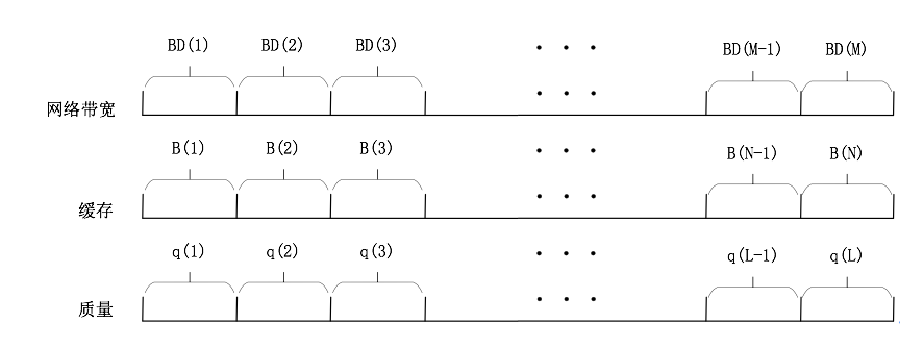
\includegraphics[width=0.8\textwidth]{q-state}
\caption{Q learning state division}
\label{q-learning state}
\end{figure*}
\begin{figure*}[ht]
\centering
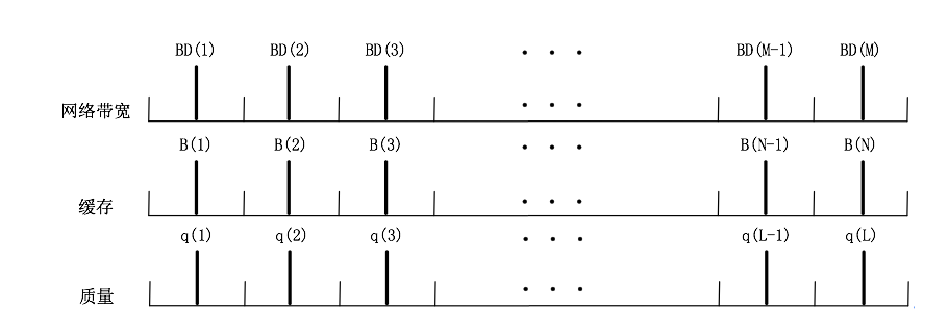
\includegraphics[width=0.8\textwidth]{knn-q-state}
\caption{KNN-Q learning state division}
\label{knn-q-learning state}
\end{figure*}
\begin{equation}
\label{state_distance}
d_{i}=\sqrt{(d_{i}^{bandwidth})^2+(d_{i}^{buffer})^2+(d_{i}^{previous-ssim})^2}
\end{equation}

After the state $s_{t}$ is obtained from the proximity state of the state in each table, 
the K minimum distance state is selected therefrom. Use their Q-value array to compute an 
array of Q values for $s_{t}$, as shown in equation \ref{Q_st}.
\begin{equation}
\label{Q_st}
Q(s_{t},:)=\left\{
\begin{array}{lr}
    Q(s_{t},:),s_{t}\in S\\
    \sum_{i=1}^K w_{i}Q(s^{(i)},a),s_{t}\notin S 
\end{array}
\right.
\end{equation}

$s_{t}\in S$ stands for $s_{t}$ in the presence table, $s_{t}\notin S$ stands for state 
$s_{t}$ not available in the status table. $s^{(i)}$ is a state adjacent to the state 
$s_{t}$. $w_i$ represents the weight of the neighboring state $s^{(i)}$. If $s^{(i)}$ 
is less than the distance $d_i$ from $s_{t}$, the larger the $w_i$. Conversely, 
if the distance of $s^{(i)}$ from $s_{t}$ is larger, the smaller the $w_i$ is, the 
specific calculation method is shown in equations \ref{w_i} and \ref{rho_i}.
\begin{equation}
\label{w_i}
w_{i}=\frac{\rho _{i}}{\sum\rho_{i}}
\end{equation}
\begin{equation}
\label{rho_i}
\rho_{i}=\frac{1}{d_{i}}
\end{equation}
\subsubsection{Q table update}
After the execution of the action is completed, the Q table needs to be updated 
based on the returned reward and the new state. If the current state can be 
found in the state partition table, the Q table is updated using equation \ref{q table update rule}. 
If the current state cannot be found in the state partition table, the Q values 
of the K adjacency states in the Q table are updated,as shown in equation \ref{knn q table update}.
\begin{equation}
\label{knn q table update}
Q(s^{(i)},a)_{t+1}\leftarrow Q(s^{(i)},a)_{t}+\lambda\theta w_{i}
\end{equation}

Among them, the calculation method of $\theta$ is shown in equation \ref{theta}. 
$s^{(i)^{\prime}}, i=1, ..., K$ is the K state adjacent to the state $s_{t}$ next state. 
The pseudo code of the bir rate adaptive algorithm based on KNN-Q learning in the training stage is shown in Table \ref{KNN-Q training}.
\begin{equation}
\label{theta}
\theta=R_{total}^{(s,a)}+\gamma max x_{a^\prime}\sum w_{i}^{\prime}Q(s^{(i)^{\prime}},a^{\prime})-\sum w_{i}Q(s^{(i)},a)
\end{equation}
\begin{table*}[htbp]
\renewcommand\arraystretch{0.8}
\centering
\caption{KNN-Q training algorithm pseudo code}
\label{KNN-Q training}
\begin{tabular}{l}
\toprule 
\textbf{Input}:The current environment information\\
\textbf{Output}:The learned Q table\\
\midrule 
1.\textbf{Initialize}:  \textbf{SET} Q(S,A) arbitrarily;\\
2.\textbf{REPEAT}(for each episode)\\     
3.\hspace{1cm}$s_{t}$ = Observe current state;\\
4.\hspace{1cm}\textbf{REPEAT}(for each step of episode)\\
5.\hspace{2cm}Choose Q value array Q($s_{t}$,:) from Q(S,A) with formula (11)\\
6.\hspace{2cm}Confirm bitrate to download with Q( ,:) using $\varepsilon$-greedy policy\\
7.\hspace{2cm}Request to download the video segment of the bitrate above;\\
8.\hspace{2cm}Update Buffer $buffer_{t}$ ;\\
9.\hspace{2cm}Calculate the Reward $R_{t}$ with formula (9); \\
10.\hspace{2cm}IF $s_{t}\in S$ \\
11.\hspace{3cm}Update Q(S,A) with formula (1);\\
12.\hspace{2cm}ELSE\\
13.\hspace{3cm}Update Q(S,A) with formula (15);\\
14.\hspace{2cm}END\\
15.\hspace{2cm}$s_{t+1}$ = Observe next state;\\
16.\hspace{2cm}$s_{t}$ = $s_{t+1}$;\\
17.\hspace{1cm}\textbf{UNTILE} reach the end of an epiode\\
18.\textbf{UNTILE} run out the episodes\\
\bottomrule 
\end{tabular}
\end{table*}
\section{Simulation}
In this paper, a series of simulation experiments are carried out through Matlab to 
evaluate and compare the performance of KNN-Q learning and traditional Q learning 
algorithms proposed in this paper. We use Matlab to write a program to 
simulate the process of the DASH client requesting to download and play the video to the server.
 This article sets the DASH client to simulate different scenes for different experiments 
 under different bandwidth conditions, the server has different rate video. 
 The K-value sensitivity of KNN-Q learning proposed in this paper is compared and analyzed.
\subsection{Video evaluation indicator}
It will cost lots of time to calculate the SSIM value frame by frame.
For convenience, this paper approximates the SSIM value of the 
video quality evaluation index to the polynomial \cite{RN19} with the relative 
value of the video relative bit rate as the independent variable. 
The SSIM values of video segments of different bit rates can be obtained from equations \ref{ssim_pho}, \ref{ssim_i}.
\begin{equation}
\label{ssim_pho}
\rho_{i}=log\left(\frac{R_{i}}{R_{1}}\right)
\end{equation}
\begin{equation}
\label{ssim_i}
SSIM_{i}\simeq1+d_{(1,v)}\rho_{i}+d_{(2,v)}\rho^2+d_{(3,v)}\rho^3+d_{(4,v)}\rho^4
\end{equation}
Where $R_{1}$ is the source bit rate of the video and $R_{i}$ is the bit rate compressed by the server. 
In equation \ref{ssim_i}, the vector $\left[1,d_{(1,v)},d_{(2,v)},d_{(3,v)},d_{(4,v)}\right]$ 
represents the complexity of the video.
\subsection{Test video}
In the simulation experiment, the test experiment video consists of multiple video scenes. 
The video complexity of a single video scene is constant, and each scene duration satisfies 
a random exponential distribution. The test video consists of 800 video clips, 
each of which has a content duration of 2 seconds.

The video material used to compose the test video in the simulation experiment is 
derived from the video set \cite{RN20} provided by EvalVid CIF.
The relationship between $\rho_{i}$ and SSIM values for each video clip in the 
video clip is shown in Figure \ref{Video material bit rate-quality curve}.

In this paper, five representative video materials (marked with thicker lines in 
the \ref{Video material bit rate-quality curve}) are selected from the video material library,
 and the whole test video is spliced by random combination. The five video materials are Brutta, 
 News, Bridge (far), Harbour and Husky. The complexity coefficients of the five video 
 materials obtained by the maximum likelihood estimation are shown in Table \ref{complexity coefficient matrix}.
\begin{figure}[htb]
\centering
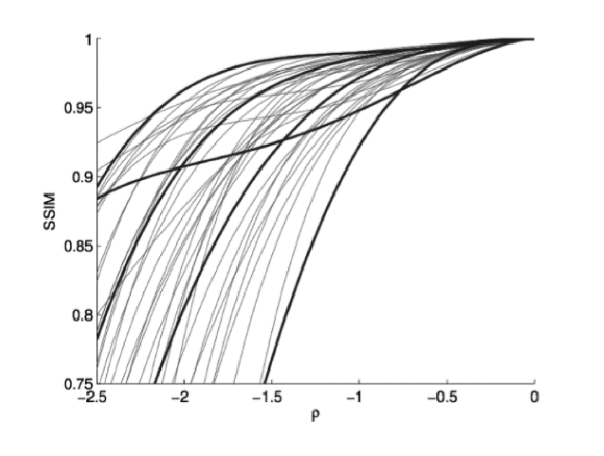
\includegraphics[width=0.8\columnwidth]{complexity}
\caption{Video material bit rate - quality curve}
\cite{RN19}
\label{Video material bit rate-quality curve}
\end{figure}
\begin{table*}[htbp]
\renewcommand\arraystretch{0.8}
\centering
\caption{Complexity coefficient matrix of 5 video materials}
\label{complexity coefficient matrix}
\begin{tabular}{cc}
\toprule 
Video name&Complexity coefficient matrix\\
&$\left[1,d_{(1,v)},d_{(2,v)},d_{(3,v)},d_{(4,v)}\right]$\\
\midrule
Brutta&[-0.0101529,-0.0288832,-0.0242726,0.0041539]\\
News&[-0.0106444,-0.0229079, -0.0253096, 0.0007417]\\
Bridge(far)&[-0.01050829,-0.0538481, -0.0821086, 0.0136133]\\
Harbour&[-0.0050534,0.0055396, -0.01726018, 0.0002203]\\
Husky&[0.0099785,0.0759046,-0.0113807,0.0003986]\\
\bottomrule 
\end{tabular}
\end{table*}
\begin{table*}[htb]
\renewcommand\arraystretch{0.8}
\centering
\caption{SSIM value at each bit rate of the video clip 5}
\label{the SSIM value at each bit rate of 5 video materials}
\begin{tabular}{ccccccccc}
\toprule 
\diagbox{Video}{Bit rate}&10000&6000&4000&3000&2000&1000&500&300\\
\midrule
Brutta&1&0.99765&0.99554&0.99403&0.99215&0.98977&0.98750&0.98425\\
News&1&0.99851&0.99657&0.99487&0.99209&0.98591&0.97584&0.96352\\
Bridge(far)&1&0.99382&0.98504&0.97767&0.966578&0.94795&0.93211&0.92284\\
Harbour&1&0.99880&0.99647&0.99376&0.98808&0.97169&0.94359&0.91266\\
Husky&1&0.99838&0.99334&0.98641&0.97046&0.92216&0.84148&0.758424\\
\bottomrule 
\end{tabular}
\end{table*}
\subsection{Simulation experiment parameter}
\begin{table}[htbp]
\centering
\renewcommand\arraystretch{0.8}
\caption{Simulation experiment general parameter}
\label{general parameters}
\begin{tabular}{cc}
\toprule 
Parameter name&Value\\
\midrule
$\eta$&0.3\\
$\lambda$&0.95\\
$\varepsilon$&0.3\\
K&2\\
$B_{max}$&20sec\\
TrainEpisodes&50\\
TestEpisodes&150\\
StepsOfEpisode&800\\
\bottomrule 
\end{tabular}
\end{table}
The values of the parameters of each scene in the simulation experiment are 
shown in the Table \ref{general parameters}. Where $\eta,\lambda$ are the learning 
rate and reward discount factor for equation \ref{q table update rule}, respectively. K is the number of 
adjacency states in KNN-Q learning, and $B_{max}$ is the upper limit of 
the buffer of the DASH client.

To avoid accidental phenomena, 10 replicate experiments were performed. 
Each set of experiments include 50 iterations of training and one test with 150 iterations. 
Each iteration includes 800 steps of training or testing.
\subsection{Experimental results and analysis}
During the download of the video by the DASH client, the buffer size 
will have an impact on QoE, and the SSIM value is also an important indicator 
for measuring video quality. When there is too much buffer, the video buffer 
will overflow the buffer area; when the buffer is too small, the buffer starvation 
will occur in the environment with poor network conditions, then the video picture will freeze.
\subsubsection{Simple scene}
The simple scene simulates a situation where the network bandwidth is relatively stable, 
but the video content is relatively simple. For example, the current user is playing a video 
of the endless blue sky, and the scene in the video is almost unchanged. Therefore, 
in the simulation experiment, only one video material News is used in this scene to 
generate a test video with a single complexity.The range of network bandwidth changes 
in a simple scene is $\left[5000,6000\right]$ kb/s.

The comparison between the buffer and video quality of the DASH client in a simple scene 
is shown in \ref{simple_buffer_compare} and \ref{simple_buffer_bar_graph}.
In a simple scene, the rate-adaptive algorithm based on KNN-Q learning has the same 
growth trend as the adaptive algorithm of traditional Q-learning, but the average 
buffer of 10 experiments is not as large as the adaptive algorithm based on Q-learning.

In a simple scene, as shown in \ref{simple_ssim_compare} and \ref{simple_ssim_bar_graph},
the average video quality of the code rate adaptive algorithm 
based on KNN-Q learning is higher than that of the traditional Q learning.
\begin{figure}[htbp]
\centering
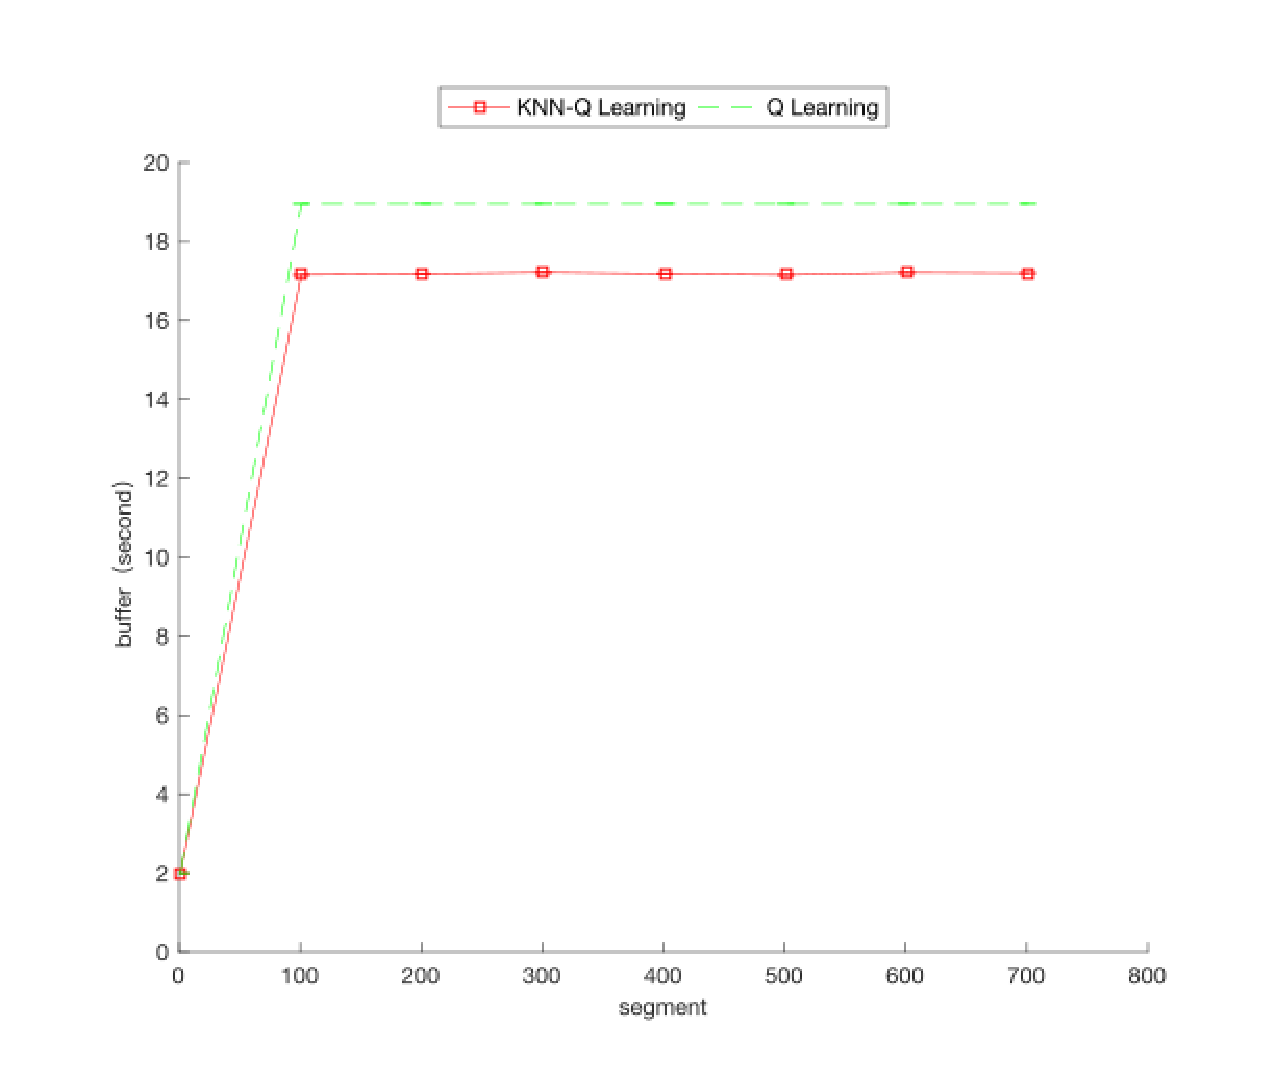
\includegraphics[width=\columnwidth]{simple_buffer_compare}
\caption{Buffer trend of simple scene}
\label{simple_buffer_compare}
\end{figure}
\begin{figure}[htbp]
\centering
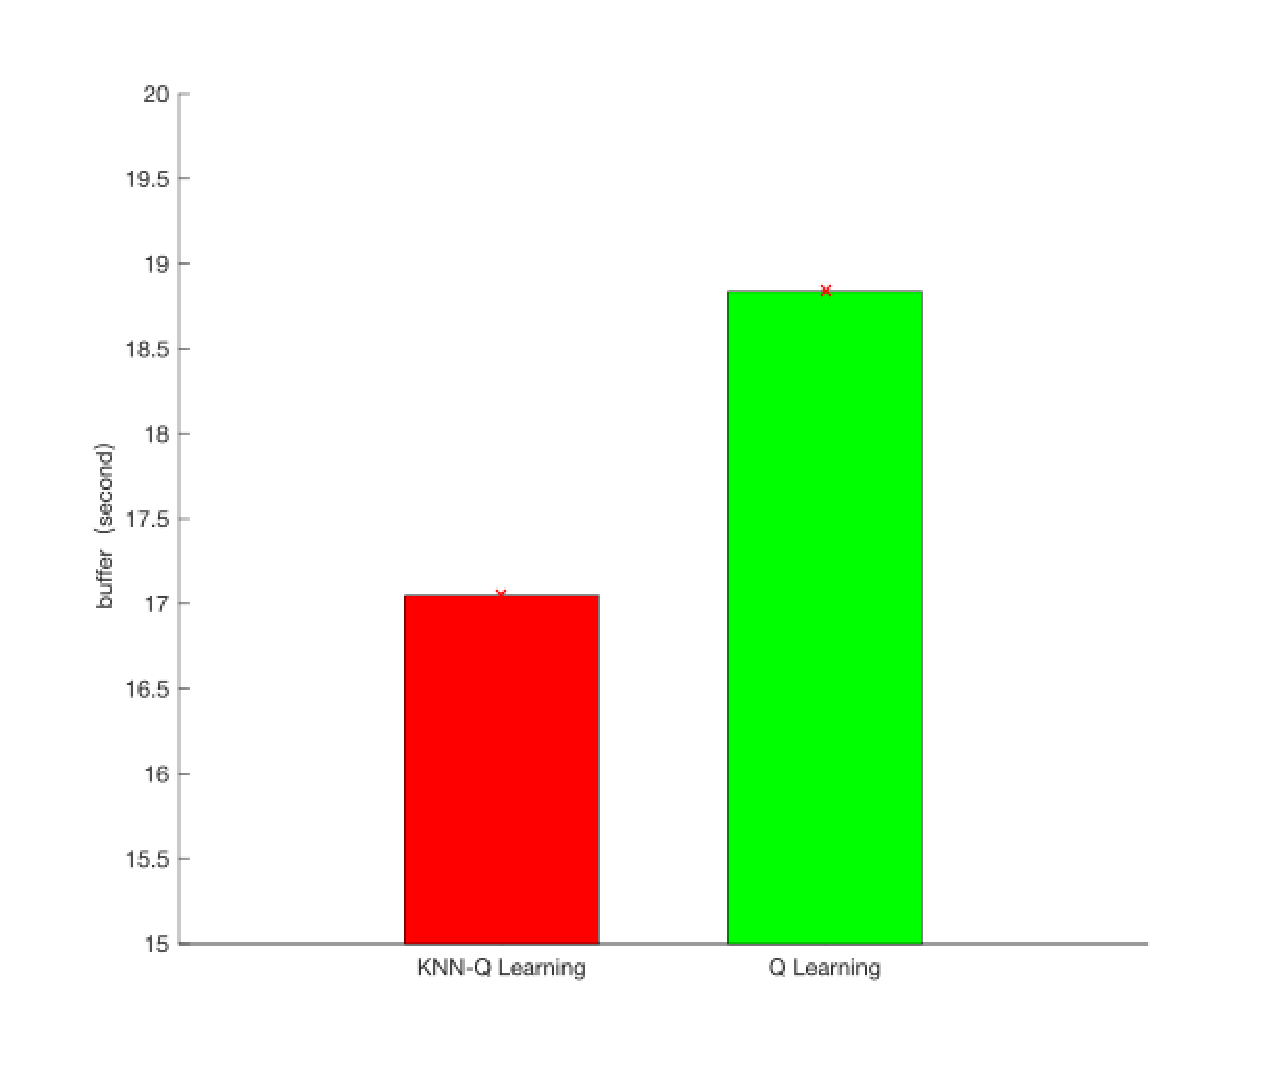
\includegraphics[width=\columnwidth]{simple_buffer_bar_graph}
\caption{Average buffer of simple scene}
\label{simple_buffer_bar_graph}
\end{figure}
\begin{figure}[htbp]
\centering
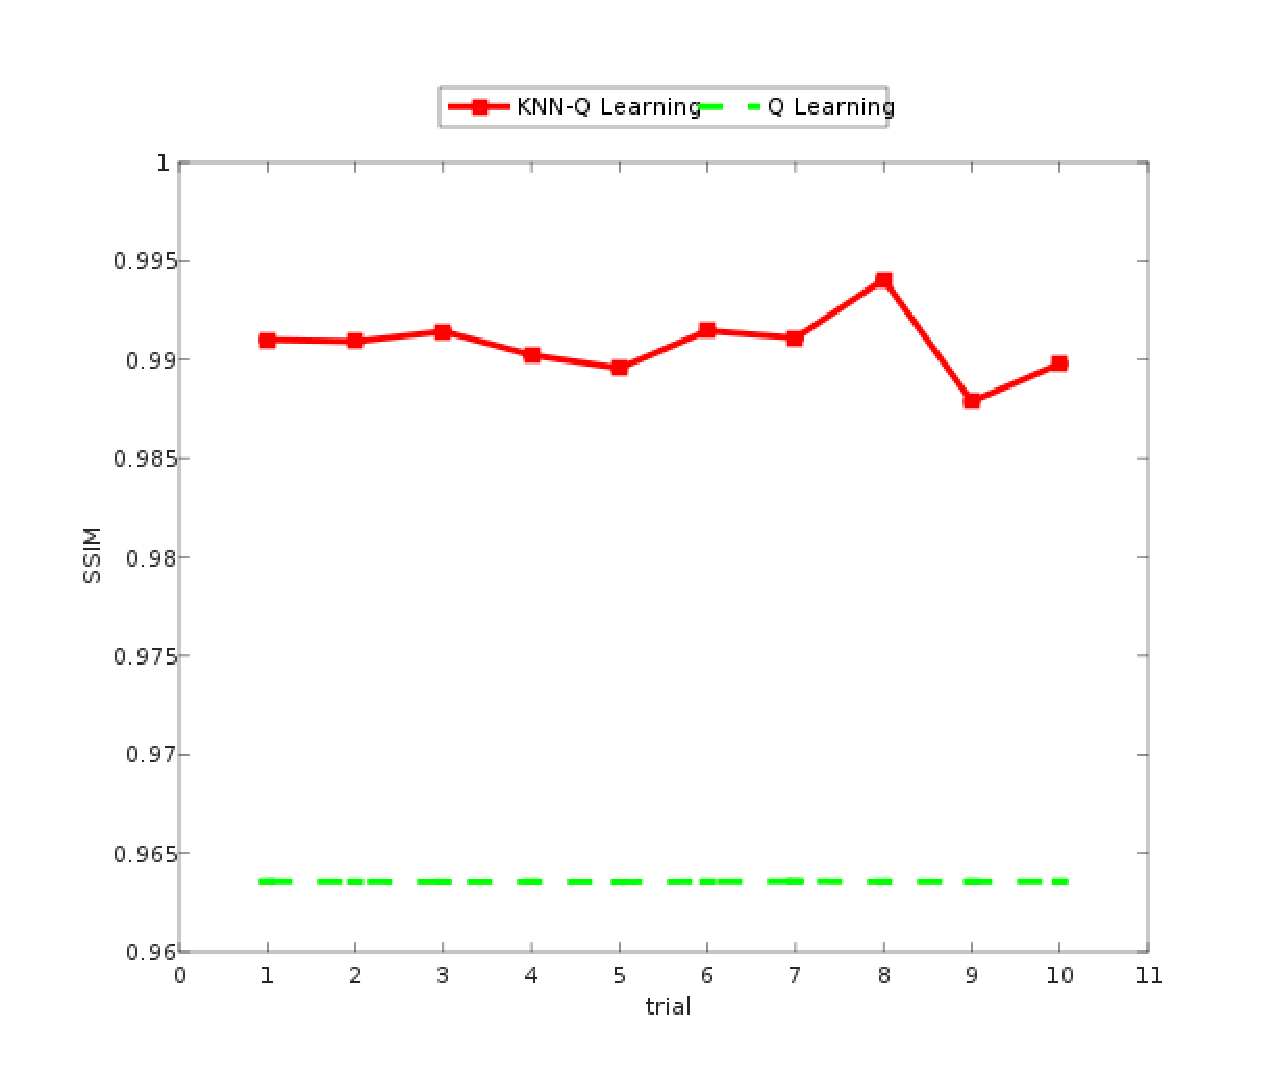
\includegraphics[width=\columnwidth]{simple_ssim_compare}
\caption{Quality comparison of simple scene }
\label{simple_ssim_compare}
\end{figure}
\begin{figure}[htbp]
\centering
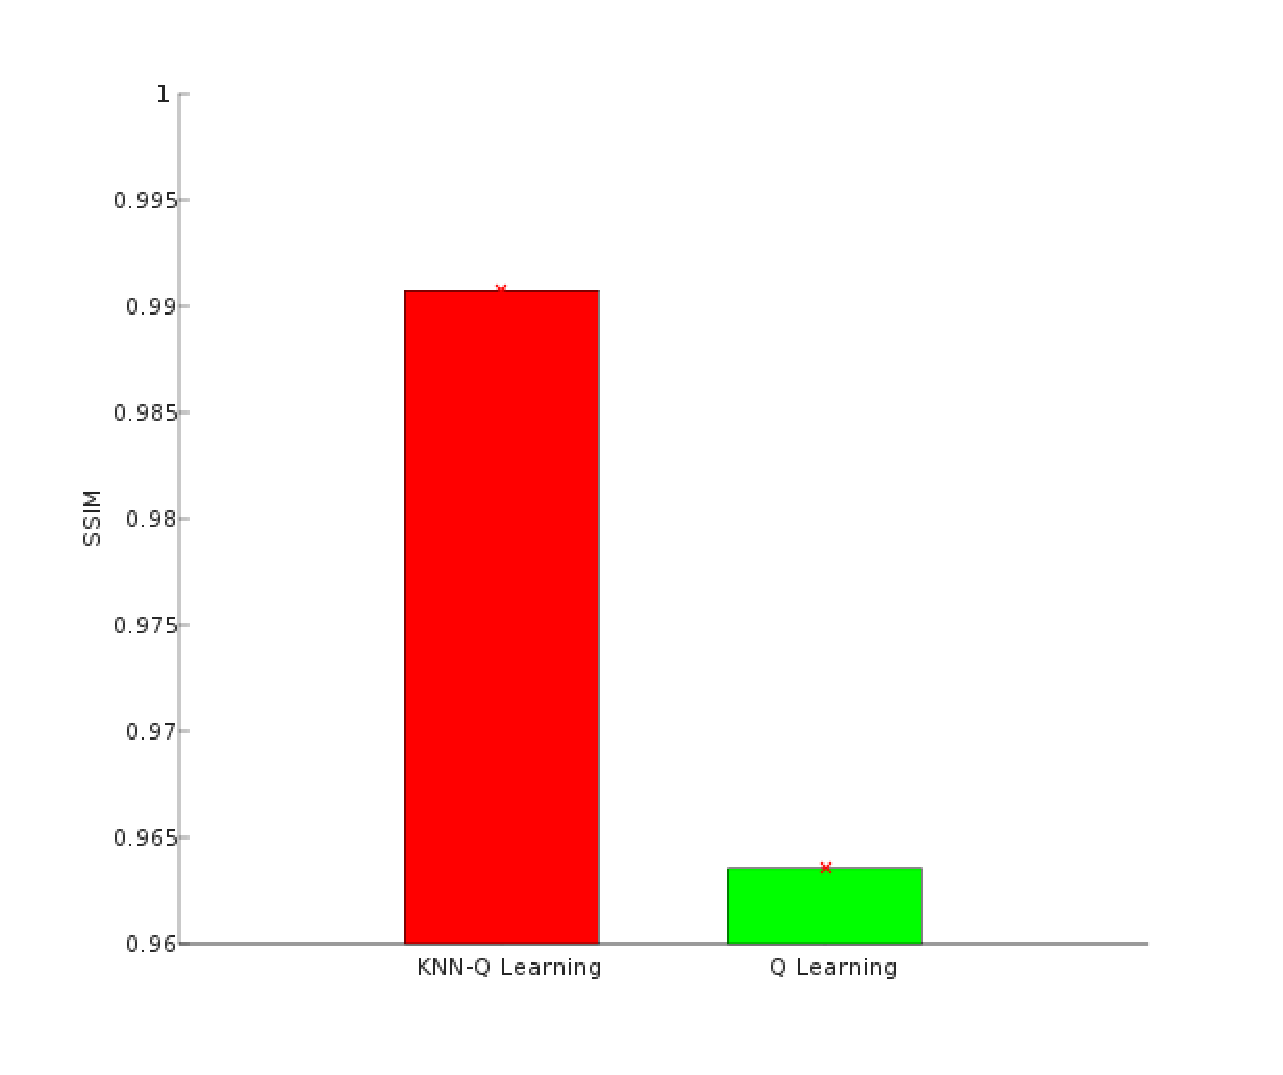
\includegraphics[width=\columnwidth]{simple_ssim_bar_graph}
\caption{Average quality of simple scene}
\label{simple_ssim_bar_graph}
\end{figure}
\subsubsection{Regular scene}
The regular scene simulation shows the playing video scene in life, 
that is, the user bandwidth is relatively stable, and the content played 
by the user is relatively rich.In the regular scene, the video video with the complexity 
of the video is generated using the five video clips in Table \ref{the SSIM value at each bit rate of 5 video materials}. 
The network bandwidth varies from $\left[5000,6000\right]$ kb/s.

It can be seen from the Figure \ref{regular_ssim_compare} and \ref{regular_ssim_bar_graph} that in the regular scene, 
the buffer growth trend of KNN-Q learning and traditional Q learning is the same.
But the 10 average experiments are not bufferd based on Q learning, and the difference between the two is nearly 7s.

It can be seen from the Figure \ref{regular_ssim_compare} and \ref{regular_ssim_bar_graph} that in the regulr scene, 
the average video quality of the bit rate adaptive algorithm based on KNN-Q 
learning is higher than that of the traditional Q learning.
\begin{figure}[htbp]
\centering
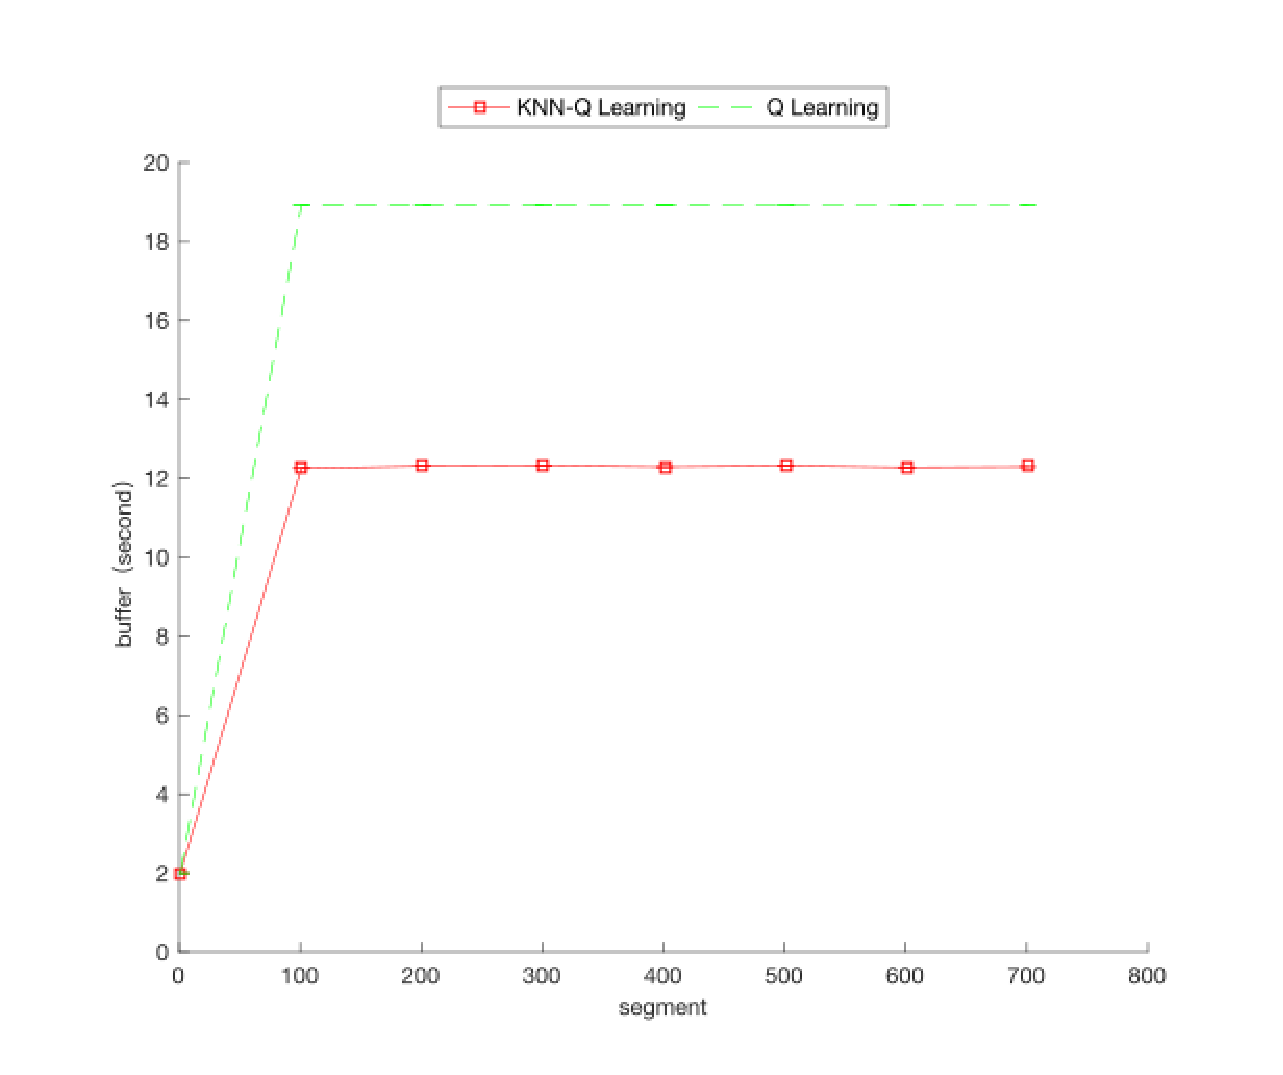
\includegraphics[width=\columnwidth]{regular_buffer_compare}
\caption{Buffer trend of regular scene}
\label{regular_buffer_compare}
\end{figure}
\begin{figure}[htbp]
\centering
\includegraphics[width=\columnwidth]{regular_buffer_bar_graph}
\caption{Average buffer of regular scene}
\label{regular_buffer_bar_graph}
\end{figure}
\begin{figure}[htbp]
\centering
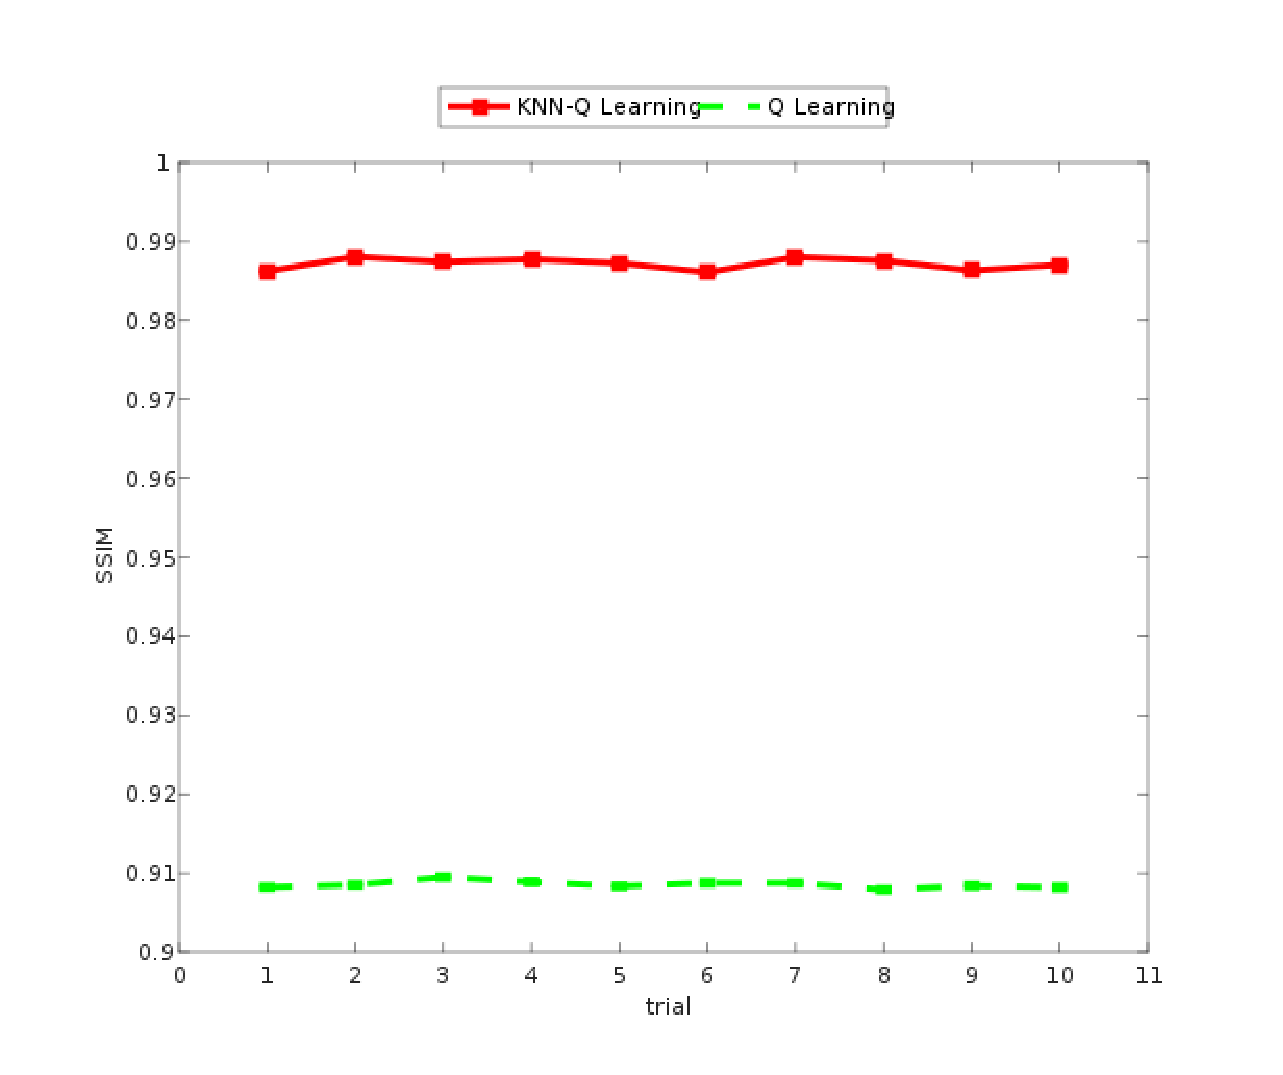
\includegraphics[width=\columnwidth]{regular_ssim_compare}
\caption{Quality comparison of regular scene}
\label{regular_ssim_compare}
\end{figure}
\begin{figure}[htbp]
\centering
\includegraphics[width=\columnwidth]{regular_ssim_bar_graph}
\caption{Average quality of regular scene }
\label{regular_ssim_bar_graph}
\end{figure}
\subsubsection{Complex scene}
The complex scene simulates the situation in which real-life network 
bandwidth fluctuations are large and video content is rich. 
In the simulation experiment, the range of the simulated bandwidth in 
the complex scene is $\left[400,12500\right]$kb/s, and the test video is 
randomly synthesized from the five video materials in Table \ref{the SSIM value at each bit rate of 5 video materials}.

It can be seen from Figure \ref{complex_buffer_compare} and \ref{complex_ssim_bar_graph} that in a complex scene, 
the buffer growth trend of KNN-Q learning and traditional Q learning is the same, 
but the 10 average experiments are not as large as the Q-based buffer.

It can be seen from the Figure \ref{complex_ssim_compare} and \ref{complex_ssim_bar_graph} that in the complex scene, 
the average video quality of the bit rate adaptive algorithm based on 
KNN-Q learning is higher than that of the traditional Q learning, and the average SSIM value is close to 0.08.
\begin{figure}[htbp]
\centering
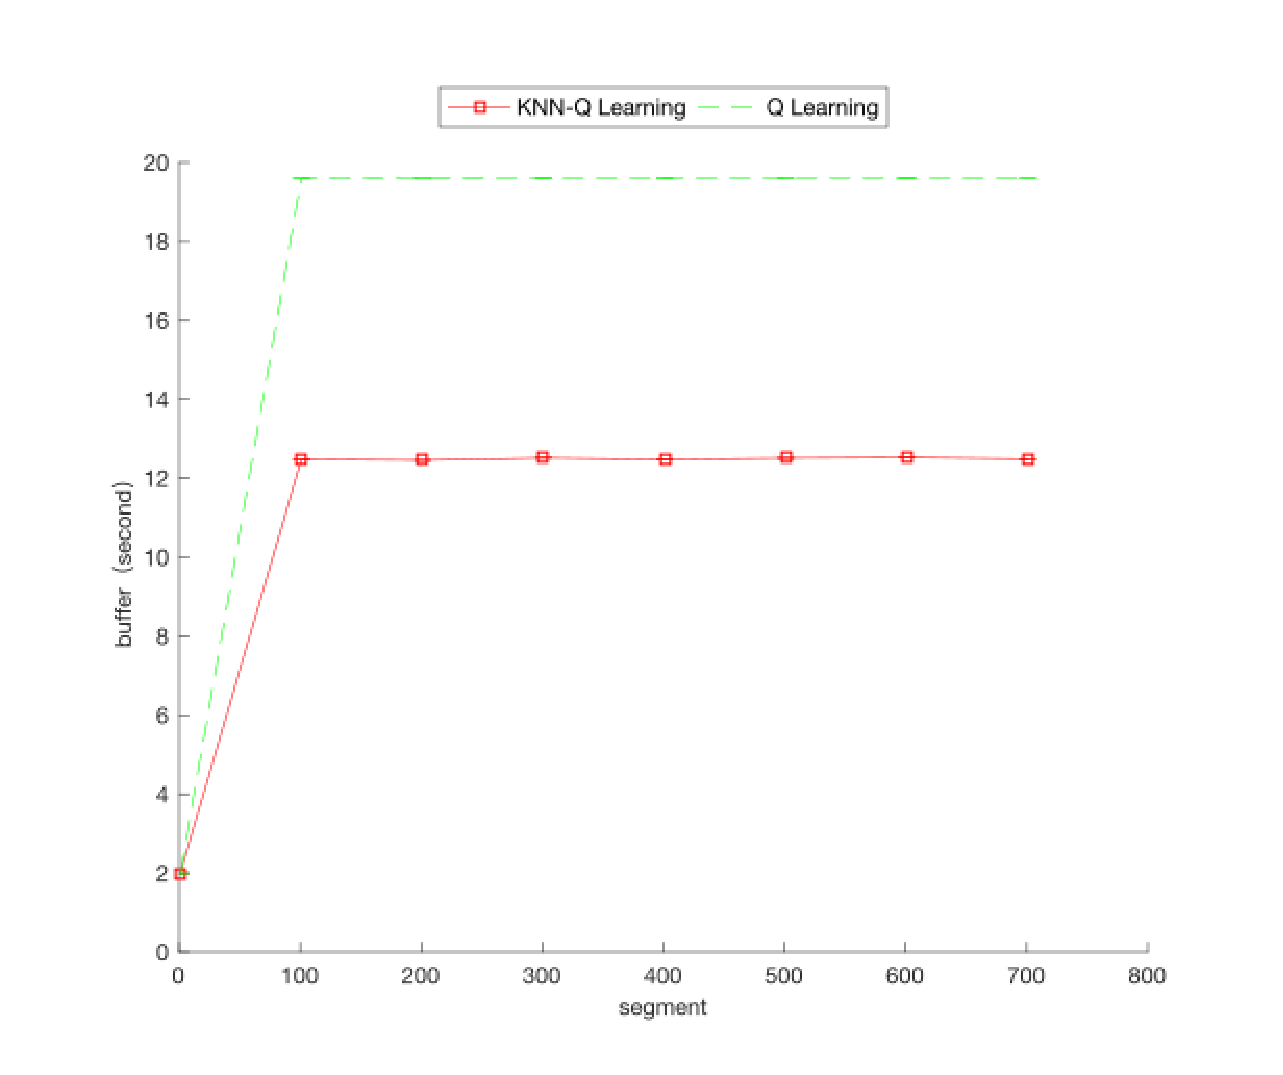
\includegraphics[width=\columnwidth]{complex_buffer_compare}
\caption{Buffer trend of complex scene }
\label{complex_buffer_compare}
\end{figure}
\begin{figure}[htbp]
\centering
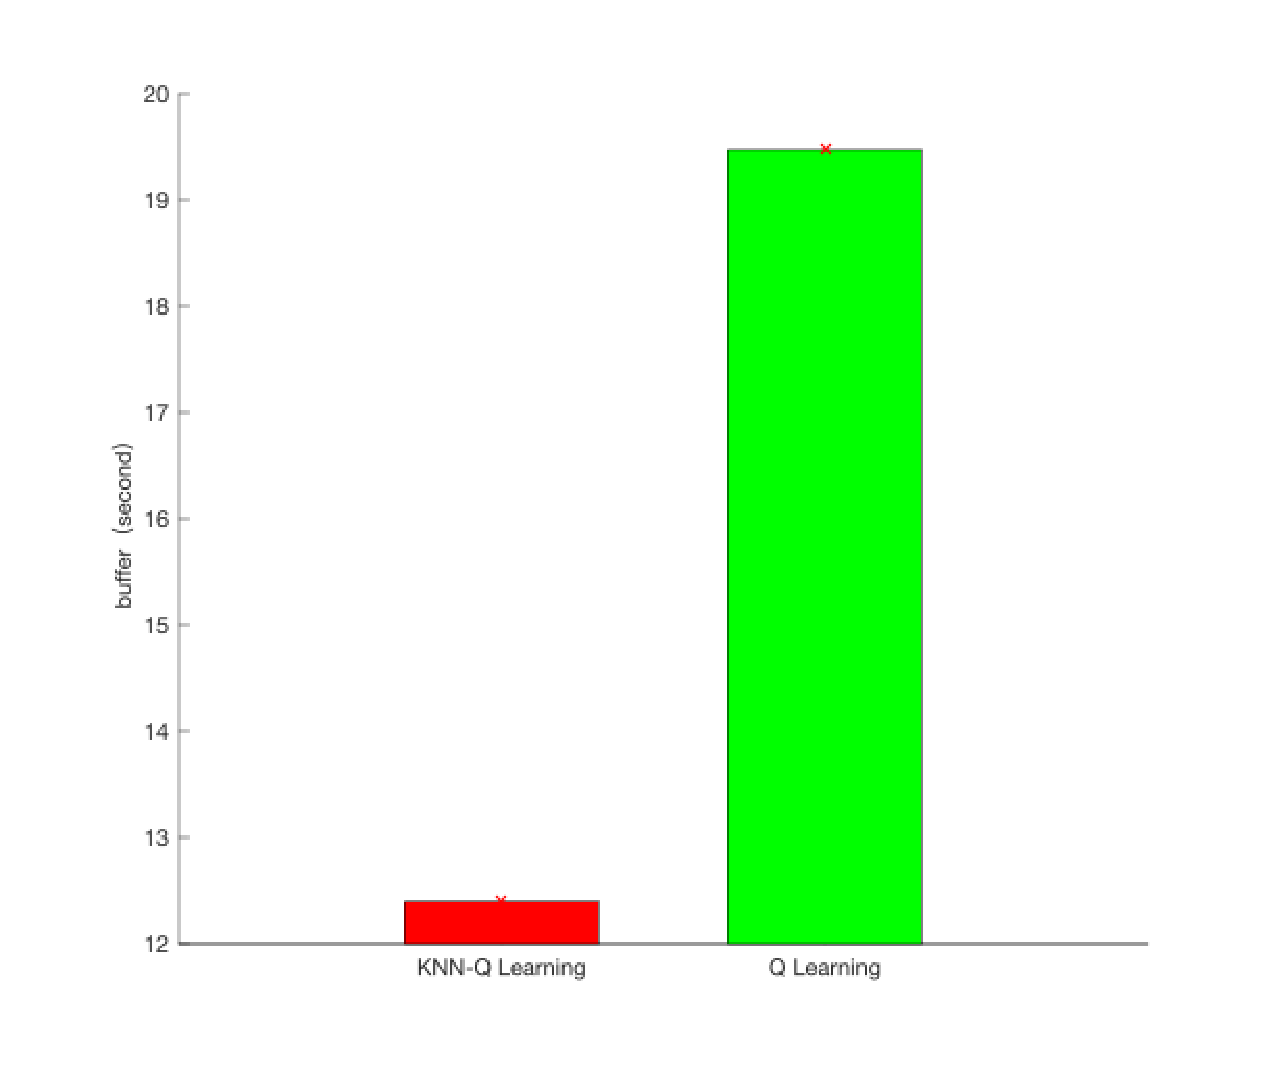
\includegraphics[width=\columnwidth]{complex_buffer_bar_graph}
\caption{Average buffer of complex scene}
\label{complex_buffer_bar_graph}
\end{figure}
\begin{figure}[htbp]
\centering
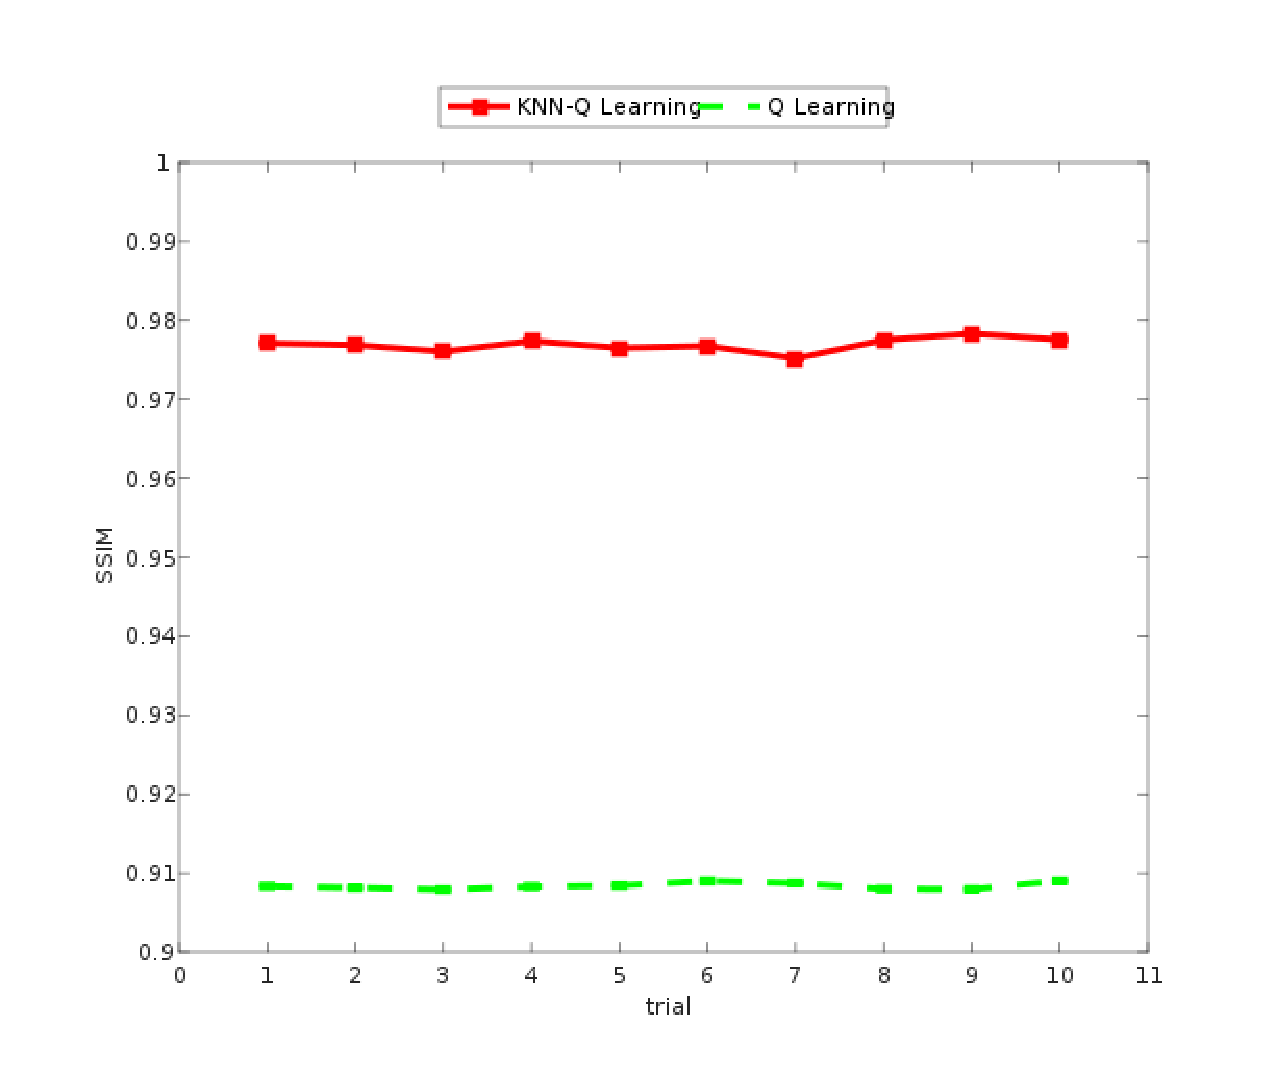
\includegraphics[width=\columnwidth]{complex_ssim_compare}
\caption{Quality comparison of Complex scene}
\label{complex_ssim_compare}
\end{figure}
\begin{figure}[htbp]
\centering
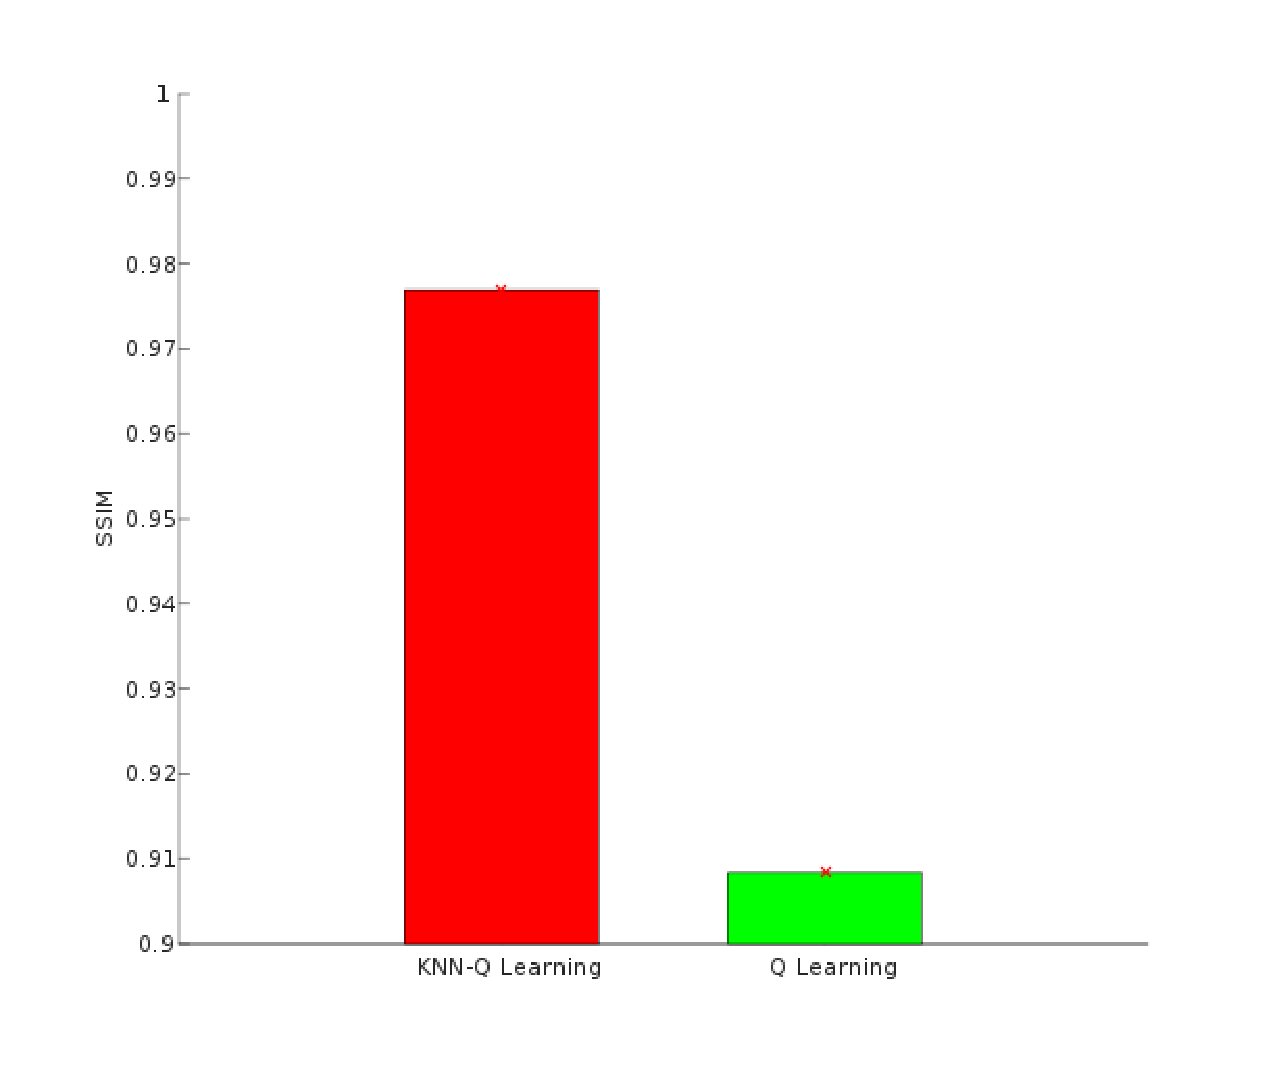
\includegraphics[width=\columnwidth]{complex_ssim_bar_graph}
\caption{Average quality of complex scene}
\label{complex_ssim_bar_graph}
\end{figure}
\subsubsection{The sensitivity of K}
In the regular scene, set the distance formula to the Euclidean distance, 
and take K = 2, 3, 4, 5, and 6 to determine the influence of the K value in KNN-Q on the 
experimental results. The test video was randomly synthesized from the five videos in 
Table \ref{the SSIM value at each bit rate of 5 video materials}. 
As can be seen from Figure \ref{k_sensitivity_buffer}, the larger the K value, the larger the buffer. 
As can be seen from Figure \ref{k_sensitivity_ssim}, the larger the K value, the smaller the average 
value of the SSIM and the worse the video quality. Especially when K=6, the 
average SSIM value drops rapidly to below 0.91.
\begin{figure}[htbp]
\centering
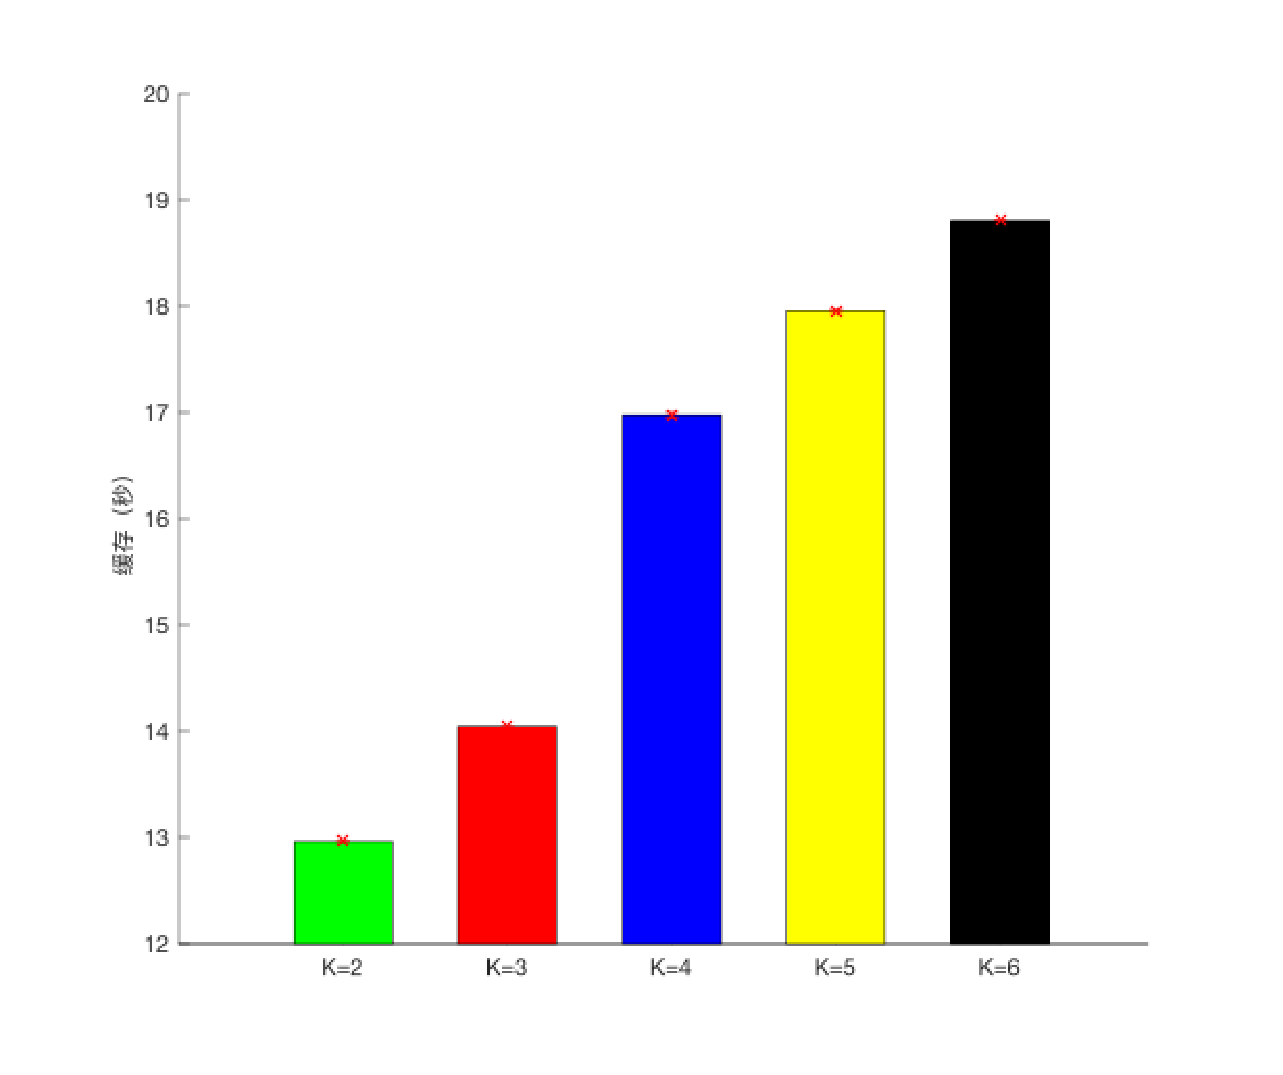
\includegraphics[width=\columnwidth]{k_sensitivity_buffer}
\caption{The effect of K value on the buffer}
\label{k_sensitivity_buffer}
\end{figure}
\begin{figure}[htbp]
\centering
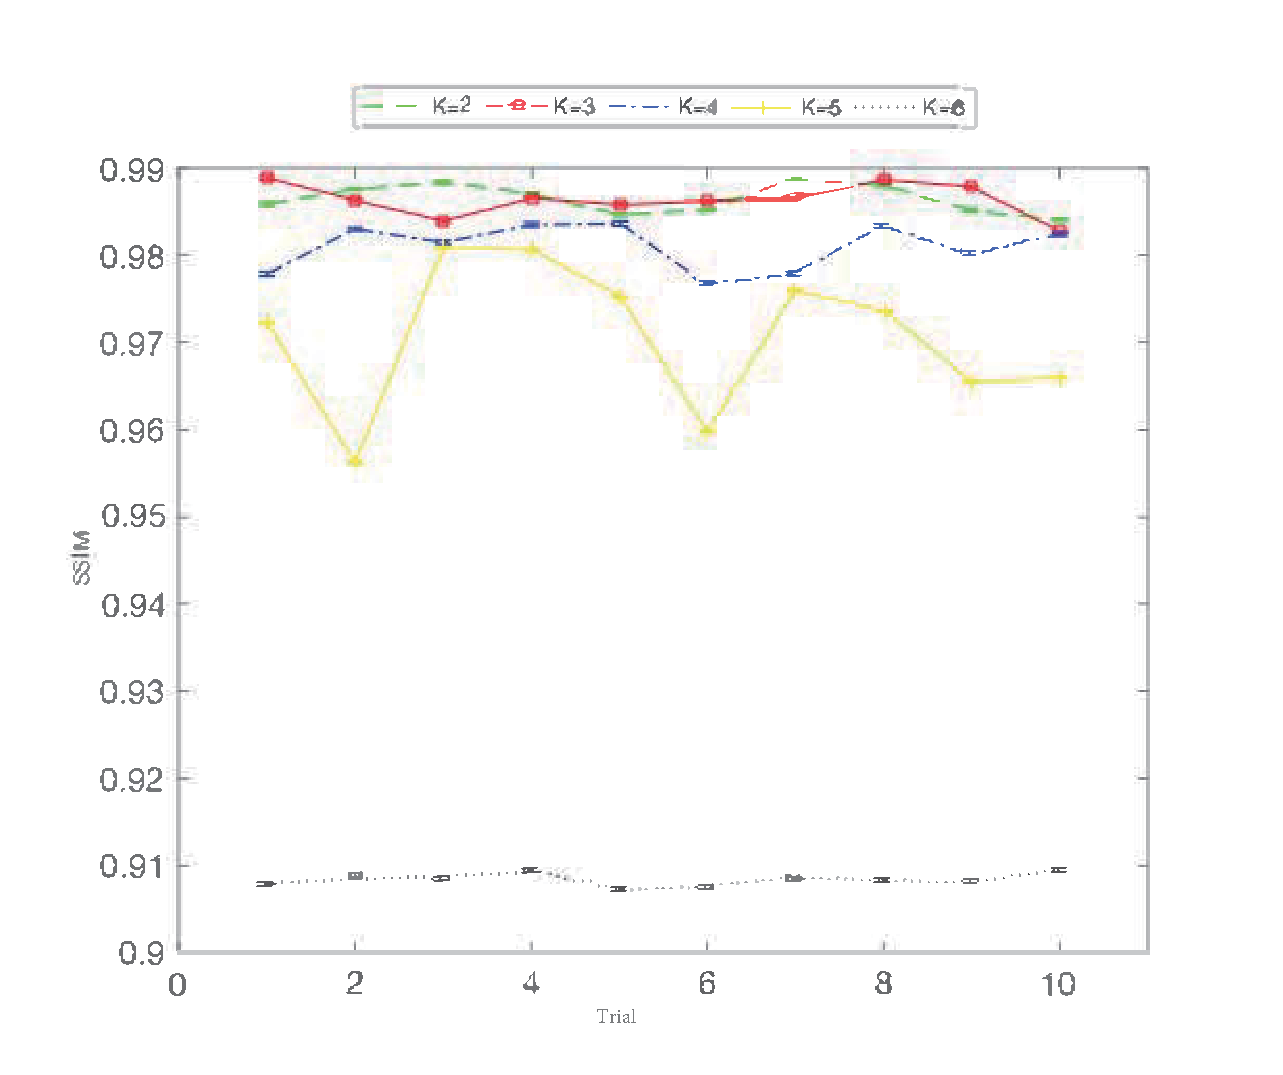
\includegraphics[width=\columnwidth]{k_sensitivity_ssim}
\caption{The effect of K value on video quality}
\label{k_sensitivity_ssim}
\end{figure}
\subsubsection{Distance formula sensitivity}
In normal scenario, we set 2 as distance. 
Euclidean distance formula, Manhattan distance formula and Chebyshev distance formula 
are used as distance formula in KNN-Q learning to judge the influence 
of distance formula on experimental results.

As shown in \ref{distance_buffer}, the three distance formulas have little effect 
on the buffer. As shown in the diagram \ref{distance_ssim}, when the distance formula
 is the Chebyshev formula, the SSIM value is the lowest, and the SSIM value is 
 the highest when using the Euclidean distance, followed by the Manhattan distance.
\begin{figure}[htbp]
\centering
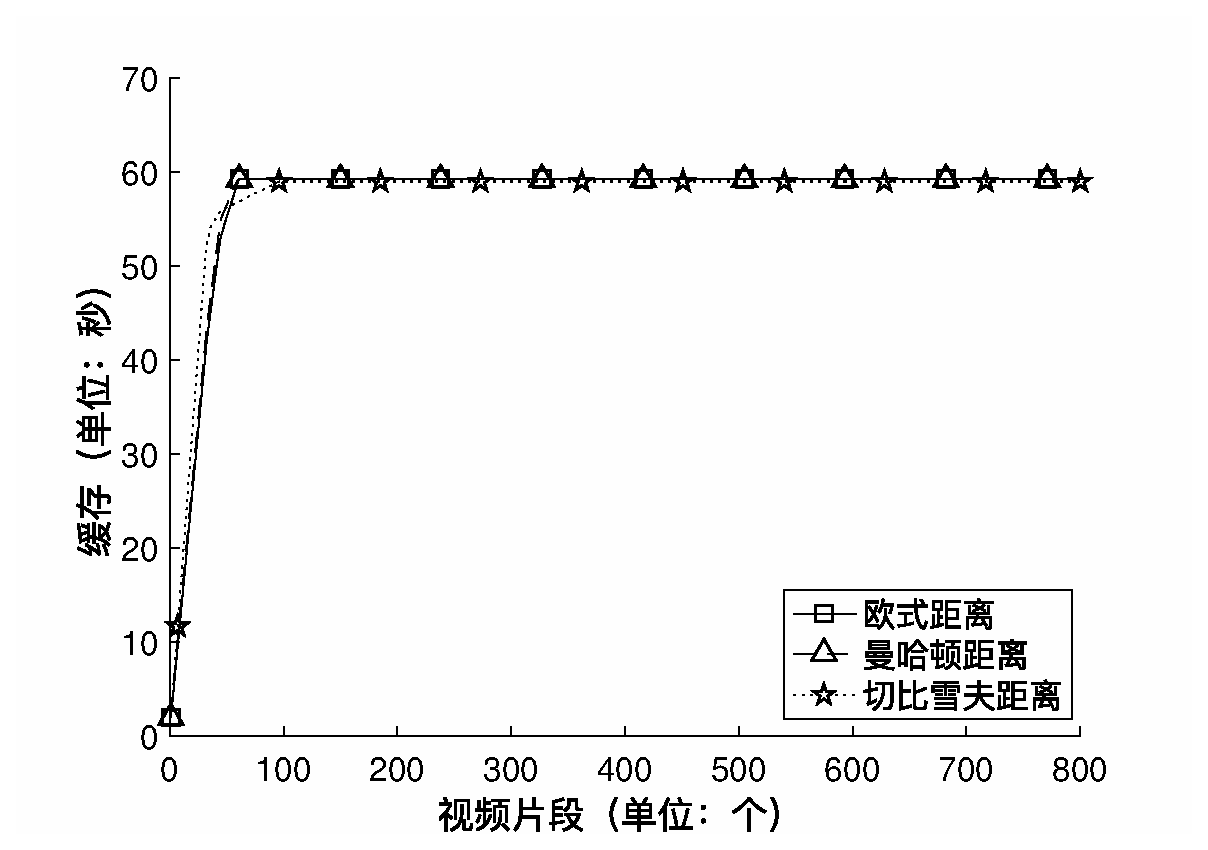
\includegraphics[width=\columnwidth]{distance_buffer}
\caption{Distance formula affects the buffer}
\label{distance_buffer}
\end{figure}
\begin{figure}[htbp]
\centering
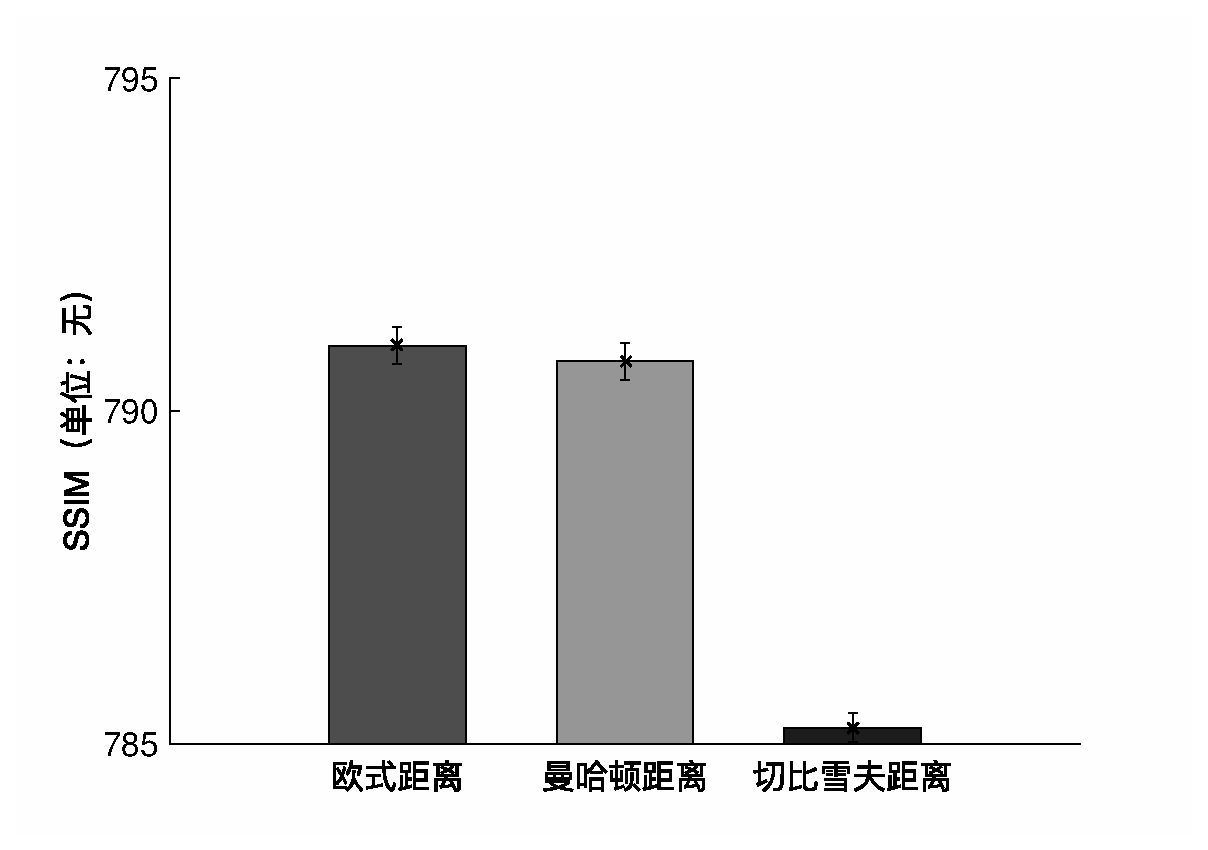
\includegraphics[width=\columnwidth]{distance_ssim}
\caption{Distance formula affects video quality}
\label{distance_ssim}
\end{figure}
\section{Conclusion}
The Matlab simulation results show that the KNN-Q learning rate adaptive 
algorithm proposed in this paper can obtain higher video quality than 
the traditional Q learning rate adaptive algorithm in simple scenes, regular 
scenes and complex scenes. In the process of training DASH client adaptive strategy, 
the convergence speed of KNN-Q learning is significantly better than traditional Q learning. 
In the process of distance and formula sensitivity test, when the Euclidean distance is used
and the distance K is 2, the algorithm can obtain higher QoE.

Subsequent attempts will be made to introduce neural networks to 
replace discrete Q tables to characterize continuous state values.
\bibliographystyle{apacite}
\bibliography{mybib.bib}
\bigskip
\end{document}

